\documentclass[10pt,fleqn,twoside]{book}
\topmargin=3cm

%cambiar fuente defecto
\usepackage{helvet}
%\renewcommand{\normalfont}{\sfdefault}

\usepackage{amsmath, amsfonts, psfrag, fancyhdr, layout, appendix, subfig}
\usepackage{graphicx}

\usepackage[utf8]{inputenc}
\usepackage[spanish]{babel}
\usepackage{makeidx}
%\usepackage{ucs}


\usepackage{color}

\definecolor{lightgray}{rgb}{0.83,0.83,0.83}
\definecolor{darkgray}{gray}{0.40}

%Colores predefinidos para usar con listing
\definecolor{code_fg}{RGB}{50,50,50}
\definecolor{code_bg}{RGB}{240, 255, 225}
\definecolor{code_coment}{RGB}{0, 80, 0} 
\definecolor{code_keyword}{RGB}{0, 50, 100}
\definecolor{code_indetif}{RGB}{0, 128, 255}
\definecolor{code_number}{RGB}{80, 80, 80}
\definecolor{console_bg}{RGB}{0, 79, 117}
\definecolor{console_fg}{RGB}{250, 250, 250}
\definecolor{console_key}{RGB}{0, 79, 157}

%color de los enlaces
\definecolor{link}{RGB}{0, 79, 157}

\usepackage[sort&compress]{natbib}

%Para bibliogafía por capítulos con BibTeX
%\usepackage[sectionbib]{natbib}
%\usepackage{chapterbib}

%This change labels of subfig
\renewcommand{\thesubfigure}{\alph{subfigure}\arabic{subfiggroup}}
\captionsetup[subfigure]{labelformat=simple,labelsep=colon,
                         listofformat=subsimple}
%\captionsetup{lofdepth=2} This is in order to list the subfigures in the LOF
\makeatletter
 \renewcommand{\p@subfigure}{}
  %Esto lo agrego yo para tener subfiguras a1, b1, ... a2, b2, ... 
  %Se reinicia cada vez que una nueva figura es convocada (como es debido).
  \newcounter{subfiggroup}[figure] 
\makeatother

\usepackage{epsfig}

%Esto genera enlaces en el PDF
\usepackage{url}

%cambiar margenes
\def\changemargin#1#2{\list{}{\rightmargin#2\leftmargin#1}\item[]}
\let\endchangemargin=\endlist


% \usepackage{html}
%Esto es para el conversor latex2html

%Este mejora las prestaciones de "\verbatim" que sirve para poner texto preformateado y en fuente monospace tipo maquina de escribir, dentro del ambito de verbatim no se reconoce ningun comando de latex
%\usepackage{verbatim}
%no uso verbatim, uso fancyvrb que da mas opciones de configuracion, se usa begin{Verbatim} end{Verbatim}
%un manual completo de fancyvrb en
%http://citeseerx.ist.psu.edu/viewdoc/download?doi=10.1.1.169.9130&rep=rep1&type=pdf
%\usepackage{fancyvrb}
%configuracion global de fancyvrb
%\fvset{
%    gobble=2, 
%    frame=leftline, 
%    framesep=3mm, 
%    fontsize=\small, 
%    formatcom=\color{darkgray}
%}

%Definición de margenes
\usepackage[left=4.5cm,top=3cm,right=2cm,bottom=2.5cm]{geometry}
\sloppy
\pagestyle{empty}

% Code for creating empty pages
% No headers on empty pages before new chapter
\makeatletter
\def\cleardoublepage{\clearpage\if@twoside \ifodd\c@page\else
    \hbox{}
    \thispagestyle{plain}
    \newpage
    \if@twocolumn\hbox{}\newpage\fi\fi\fi}
\makeatother \clearpage{\pagestyle{plain}\cleardoublepage}

% Code for creating fully-empty pages
% Fully empty pages before command is called
\makeatletter
\def\clearfullypage{\clearpage\if@twoside \ifodd\c@page\else
    \hbox{}
    \thispagestyle{empty}
    \newpage
    \if@twocolumn\hbox{}\newpage\fi\fi\fi}
\makeatother \clearpage{\pagestyle{empty}\clearfullypage}

% Dutch style of paragraph formatting, i.e. no indents.
\setlength{\parskip}{1.3ex plus 0.2ex minus 0.2ex}
\setlength{\parindent}{0pt}


% Double space for REVISION
%\renewcommand{\baselinestretch}{2.0}

%Print subsubsection numbers and put them in TOC
\setcounter{secnumdepth}{3}
\setcounter{tocdepth}{3}

\makeindex

%enlaces web en pdf remplazado por url
\usepackage{hyperref}

\hypersetup{
    colorlinks=true,
    linkcolor=black,
    urlcolor=link
}


%listings reconoce la sintaxis de varios lenguajes y permite otras configuraciones.
\usepackage{listings}
%listing definicion para formateo de codigo fuente
\lstdefinestyle{Python}
{
    basicstyle=\small\ttfamily\color{code_fg},
    backgroundcolor=\color{code_bg},
    keywordstyle=\color{code_keyword}\tt, % underlined bold black keywords
	identifierstyle=\color{code_indetif}, % color identificadores
	commentstyle=\color{code_coment},                       % comentarios
	stringstyle=\ttfamily,                                 % typewriter type for strings
	showstringspaces=false,
	frame=shadowbox,%\linewidth=3,
	framexleftmargin=8mm,
	rulesepcolor=\color{code_fg},
	backgroundcolor=\color{code_bg},
	language=Python, 
	numbers=left, 
	numberstyle=\color{code_number}\footnotesize\tt,		%estilo numero linea
	tabsize=4, 						                        %tamaño tabulacion 	    
	%showspaces=true,
}

\lstdefinestyle{HTML}
{
    basicstyle=\small\ttfamily\color{code_fg},
    backgroundcolor=\color{code_bg},
    keywordstyle=\color{code_keyword}\tt, % underlined bold black keywords
	identifierstyle=\color{code_indetif}, % color identificadores
}

\lstdefinestyle{consola}
{
    basicstyle=\ttfamily\color{console_fg},
    backgroundcolor=\color{console_bg},
}


%FIN Definicion para Formateo Codigo

\usepackage{lmodern}% http://ctan.org/pkg/lm 

\begin{document}


%Cambiar Cuadros por Tablas y lista de... Debe ir después de \begin{document}
%\renewcommand{\listtablename}{Índice de tablas} 
%\renewcommand{\tablename}{Tabla} 


\pagenumbering{arabic}

%%%%%%%%%%%%%
\frontmatter
%%%%%%%%%%%%%
%\ input{portada} %Se compila aparte y se junta con "gs".
%gs -dNOPAUSE -sDEVICE=pdfwrite -sOUTPUTFILE=tesiscompleta.pdf -dBATCH portada.pdf tesis.pdf
\pagestyle{empty}
\clearfullypage


% Define pagestyle
\pagestyle{fancy}
\fancyhf{}
\renewcommand{\chaptermark}[1]{\markboth{ \emph{#1}}{}}
\fancyhead[LO]{}
\fancyhead[LO]{}
\fancyfoot[LE,RO]{\thepage}

% Redefine plain page style
\fancypagestyle{plain}{
\fancyhf{}
\renewcommand{\headrulewidth}{0pt}
\fancyfoot[LE,RO]{\thepage}
}

% Dutch style of paragraph formatting, i.e. no indents.
\setlength{\parskip}{1.3ex plus 0.2ex minus 0.2ex}


% Remove parskip for toc
\setlength{\parskip}{0ex plus 0.5ex minus 0.2ex}


%Portada
%\documentclass[a4paper,10pt]{report}
%\usepackage{lmodern}% http://ctan.org/pkg/lm 
%\usepackage[spanish]{babel} %espaniol
%\usepackage[latin1]{inputenc} %acentos sin codigo
%\usepackage{graphicx} 
%\topmargin=3cm

%\begin{document}


\begin{titlepage}


\begin{center}
    {\fontsize{45}{45} \selectfont 
    Sistema de Gestion de \\ Consultorios Medicos \\[2.3cm] }
\end{center}


\begin{center}
    \LARGE Universidad Nacional de Salta \\
    \begin{figure}[h]
        \begin{center}
        
\includegraphics[scale=0.5]{resourse/logo-UNSa.jpg}
        \end{center}
    \end{figure}

    
    \LARGE Facultad de Ciencias Exactas \\
    Seminario de Computaci\'on \\ [2.3cm]
\end{center}


\begin{flushright}
    \Large Alumno: Ricardo Daniel Quiroga \\
    Director de Tesis: Ernesto Sanchez \\
    Proyecto Especifico \\ 
    Febrero de 2014 
    
    
\end{flushright}



\end{titlepage}



%\chapter{Dedicatoria}


\vspace*{\fill}
\begin{changemargin}{5cm}{0.1cm}
{\sf \large \em \raggedleft
Escribiriria una bonita frase copiada de algun lado pero no se me ocurre
donde buscar algo que refleje todo el exfuerzo puesto en completar este
proyecto, mejor solo doy las gracias a todos aquellos que de una u otra forma
ayudaron durante el transcurso del mismo.
}
\end{changemargin}
\vspace*{\fill}


\newpage






\tableofcontents %Indice
\listoffigures %listado de figuras
%\listoftables

%\cleardoublepage
%\ include{resumen} 
%\cleardoublepage
%\ include{resumenen} 
% Adjustments headers
\fancyhead[RO]{\leftmark}

%%%%%%%%%%%%%
\mainmatter
%%%%%%%%%%%%%


% Adjustments headers
\fancyhead[RO]{\leftmark}
\fancyhead[EL]{\emph{Capítulo \thechapter}}
%\setcounter{page}{3}
%\ include{file} busca el archivo file.tex en el directorio actual y se lo tomo como si el contenido de
%file.tex estuviera en vez del comando \include pero insertando una pagina en blanco antes y después del 
%contenido de file.tex por lo que el al escribir file.tex hay que hacer de cuentas que se esta dentro de 
%\begin{document} del documento principal, en este caso este archivo es el principal. \input es un comando 
%similar pero no agrega las paginas en blanco  
%elimine algunos \include por que no aportan nada, el que quedo tiene algunos ejemplos de uso de fancyvrb y listings
%el espacio que queda en \ include es solo para que Texmaker no reconozca el include y lo muestre en la estructura del archivo.

\chapter{Introducci\'on}

El presente trabajo de tesis es para obtener el t\'{\i}tulo intermedio de Computador 
Universitario perteneciente a la carrera Licenciatura en An\'alisis de Sistemas (plan 97)
de la Universidad Nacional de Salta.\\[0.1cm]

El tema elegido para desarrollar corresponde a un sistema de gesti\'on para consultorios m\'edicos, 
en el se intento reflejar todos los conocimientos que adquir\'{\i} durante el cursado de 
la carrera. En cuanto a las razones para la elecci\'on del tema son entre otras, el buscar
desarrollar un sistema que por sus dimensiones se proponga como un reto, ya que hasta la 
fecha solo ten\'{\i}a experiencia en cuanto al desarrollo de peque\~nas aplicaciones. 
El \'area de aplicaci\'on quedo definida, por la simple raz\'on que ten\'{\i}a contacto
con profesionales del \'area de la Salud.\\[0.1cm]

En cuanto a tecnolog\'{\i}a quise implementarlo usando algo distinto del tradici\'on PHP 
y MySQL para Web, opte por probar una tecnolog\'{\i}a que no conoc\'{\i}a Python, Django
y PosgreSQL, la cual ten\'{\i}a bastante buenas opiniones por parte de terceros y por 
suerte no decepciono sobre todo Django, que cambio mi forma de pensar a la hora de encarar
un proyecto web.\\[0.1cm]


\section{Objetivos Generales}

El Objetivo del proyecto de tesis fue el de dise\~nar y desarrollar un Sistema Centralizado 
para el \'area Salud, espec\'{\i}ficamente aplic\'andose al \'area de consultorios m\'edicos, 
permitir un mejor seguimiento y control de la evoluci\'on de los pacientes mediante la 
informatizaci\'on de los diferentes ex\'amenes y consultas que se le realizan al paciente 
posibilitando la unificaci\'on de su historia cl\'{\i}nica. Adem\'as de tambi\'en gestionar 
la asignaci\'on de turnos a los pacientes.\\[0.1cm]

Lo que se pretende es brindar un sistema modular y eficiente que permita su f\'acil 
aplicaci\'on y adem\'as de brindar la posibilidad de modificaci\'on tanto para adecuaci\'on 
para casos espec\'{\i}ficos como extensi\'on de sus funcionalidades.\\[0.1cm]


\section{Resumen}

El ``Sistema Web de Gesti\'on de Consultorio M\'edicos", desde ahora el Sistema, esta pensado
para satisfacer las necesidades de Consultorios M\'edicos o cualquier otra actividad en donde
sea necesario almacenar informaci\'on demogr\'afica de Pacientes , Historias Cl\'{\i}nicas, 
Prescripciones as\'{\i} tambi\'en como la asignaci\'on de turnos.\\[0.1cm] 

Al Ser un Sistema Centralizado, se puede acceder al el desde cualquier navegador web actual 
que cuente con conexi\'on a Internet, lo que permite entre otras cosas:\\[0.1cm]

Disminuir los tiempos de esperas por parte de pacientes a la hora de solicitar ser atendidos, 
solo necesita solicitar un turno v\'{\i}a web el sistema autom\'aticamente le asignara una 
fecha y hora acorde a sus requerimientos. Permite a los m\'edicos manejar mas f\'acilmente su
agenda para atenci\'on de pacientes.\\[0.1cm]

Mejorar el Seguimiento de los Pacientes por parte de los m\'edicos, centralizando toda su 
informaci\'on ya que con ello el m\'edico puede monitoria la evoluci\'on de su paciente donde 
sea que se encuentre ya que solo necesitara una PC con conexi\'on a Internet.\\[0.1cm]









%\ include{antecedentes}
%\chapter{Diseño}
Acá un resumen del capitulo
\section{Bases}
Para diseñar JDBGM se tomo como idea base el patrón de desarrollo DAO
\section{JDBC y su envoltorio}
y otro
\section{Abstracción de SQL}
Así que para brindar una abstracción sobre la base de datos es necesario que las consultas SQL (sin hacer diferencias sobre DDL \footnote{Data Definition Lenguaje} y DML \footnote{Data Manipulation Lenguaje}) no sean manejadas de forma explicita es decir que no seria conveniente, por ejemplo, manejar las consultas como cadenas de caracteres ya que esta es una estructura estática dependiente del DBMS que se este usando. Por lo que para poder manejar adecuadamente las consultas se considero usar una estructura de datos un poco mas compleja que contenga la consulta de manera desglosada. Es decir que en ves de tener una sentencia como la siguiente:
%ejmplo de uso de fancyvrb
\begin{Verbatim}
  nombre_comando [parametro] opcion1 [parametro] opcion2 [parametro]; 
\end{Verbatim}

Se tendría una estructura de datos como la siguiente:
%ejemplo de uso de listing
\lstset{frame=single, rulesepcolor=\color{black}, backgroundcolor=\color{lightgray}}
\begin{lstlisting}
class Sentencia{
	nombre_comando;
	opcion1;
	opcion2;
	devolver_sentencia;
}
\end{lstlisting}

Este conjunto estará formado por:
\begin{enumerate}
\item CREATE TABLE - Permite crear tablas 
\item ALTER TABLE - Modifica la estructura de una tablas \footnote{Solo se da un soporte básico para esta sentencia}
\item UPDATE - Modifica las filas de una tabla 
\item INSERT - Inserta nuevas filas a una tabla
\item DELETE - Elimina columnas de una tabla
\item SELECT - Realiza consulta sobre las tablas
\end{enumerate}

\subsection{Diseño de CREATE TABLE}
Esta sentencia es usada para crear tablas en una base de datos relacional, un resumen de su sintaxis como se la define en el estándar SQL es la siguiente:
\begin{lstlisting}
  CREATE TABLE <table name> (
  { <column name> [ <column type> ][ PRYMARY KEY ][ REFERENCES <foreign table> ] }...
  )
  [ PRIMARY KEY <indexed columns> ]
  [ FOREIGN KEY <columns and referenced table> ]
\end{lstlisting}

Así que finalmente tenemos las siguiente sintaxis para nuestro proyecto
\begin{lstlisting}
  CREATE [ TEMPORARY ] TABLE <database name> <dot> <table name> 
  <table contents source>

  <table contents source> ::=
    <left paren> <table element> [ { <comma> <table element> }... ] <right paren>
  | AS <select stmt>

\end{lstlisting}

\subsection{Diseño de UPDATE e INSERT}
Y

%\ include{implementacion}
%\ include{ejemplo}
%\ include{conclusiones}
%\ include{trabajofuturo}
%\ include{designsvt}
%\ include{lira}
%\ include{pcnc}
%\ include{exp}
%\ include{conclusion}
%\ include{futuro}

\chapter{Instalacion y Configuracion}

En este Capitulo Aparte de guiarle para realizar una exitosa implementacion
Local del Servidor de Produccion se hara referencia a cada una de las
Herramientas y librerias Utilizadas.

\section{Requerimientos}

\subsection{Requerimientos de Hardware}

Cualquier equipo que cumpla con las Caracteristicas para correr Windows 7 es suficiente
en terminos de requerimientos minimos de Hardware siempre y cuando el numero de usarios
esperados no sea alto, despues el resto dependera de sus necesidades.\\[0.5cm]

\begin{itemize}
    \item Procesador x86, x64 de 1 Ghz o superior.
    \item Memoria Ram 1 GB o Superior 
\end{itemize}


\subsection{Requerimientos de Software}


\begin{itemize}
    \item Apache 2.2
    \item PosgreSQL 9.2
    \item Python 2.7.x o Python 2.6.x
    \item Django 1.3.x o Superior
    \item PGAdmin
    \item psycopg2
    \item mod\_wsgi
    \item ReportLab
    \item easy\_thumbnails
    \item django\_extensions
    \item django\_cron
\end{itemize}


\section{Apache}

Existen 2 caminos para instalar Apache La Primera Hacer una instalacion Limpia
de Apache, la 2da es cuando no se quiere trastear con tanta configuracion por lo que
opta por infraestructuras tipo WAMP, LAMP, WAPP, etc.

\subsection{Instalacion en Limpio}

Solo recomiendo este tipo de instalacion desde 0 para quienes ya poseen un conocimiento
avanzado en cuanto a manejo de servidores.

Descargamos de \url{Apache.org} la ultima version disponible, puedes utilizar el siguiente
vinculo: \url{http://www.apachehaus.com/cgi-bin/download.plx}. \\ 
Crea dos carpetas en la unidad C, la primera de nombre {\bfseries Apache} y la segunda
{\bfseries servidor}. Descomprime el archivo descargado y ejecútalo,
sigue los pasos de la instalación y de los datos que te piden solo escoge el
destino de la instalación, que será la carpeta que creaste en
{\bfseries C:\textbackslash Apache }, los otros datos déjalos de la forma
predeterminada para configurarlos más tarde.
El programa al instalarse crea un icono en el área de notificación que te
permitirá: iniciar, detener y reiniciar Apache; tienes que tener en cuenta que
cualquier cambio que hagas en el archivo de configuración no tendrá efecto
hasta que reinicies el servidor.

\subsection{Instalacion mediante WAMP, LAMP, MAMP, WAPP}

Existem una infinidad de Paquetes precompilados y configurados, con Apache, PHP, PosgreSQL o MySQL y mas.
Dichas infraestructuras suelen nombrarse como el acronomico de las herramientas que agrupan por ejemplo:\\[1cm]

\begin{itemize}
    \item {\large WAMP {\bfseries W}indows {\bfseries A}pache {\bfseries M}ySQL {\bfseries P}HP}
    \item {\large WAPP  {\bfseries W}indows {\bfseries A}pache {\bfseries P}osgreSQL {\bfseries P}HP}  
    \item {\large LAMP {\bfseries L}inux {\bfseries A}pache {\bfseries M}ySQL {\bfseries P}HP} 
    \item {\large MAMP {\bfseries M}ac OS {\bfseries A}pache {\bfseries M}ySQL {\bfseries P}HP}  
\end{itemize}


Algunas distribuciones mas usadas disponibles Para Windows son WAMP Server \url{http://www.wampserver.com/} (WAMP),
XAMPP \url{http://sourceforge.net/projects/xampp/} (WAMP + Perl), Bitnami \url{http://bitnami.com/stack/wapp} (WAPP)
solo nos resta elegir cualquiera de ellas e instalarlas, aparte de la ruta de instalacion nos pediran el usuario y
contraseña para acceder al motor de Base de Datos.

\subsection{Configuracion}

Toda la configuración para el funcionamiento de Apache se guarda en un archivo
de texto nombrado: {\bfseries httpd.conf} que se encuentra en la ruta
{\bfseries C:\textbackslash Apache \textbackslash conf } si realizamos una instalacion en limpio o
{\bfseries C:\textbackslash wamp \textbackslash bin \textbackslash  Apache \textbackslash conf } si
instalamos el paquete multiple preconfigurado no es necesario realizar este paso por lo
que lo podremos salta.\\

Al archivo {\bfseries httpd.conf} lo podemos editar en cualquier editor de texto como Notepad.

Buscamos la linea que dice

\begin{lstlisting}[style=consola, numbers=none]
    Listem LocalHost:80
\end{lstlisting}

y la Cambiamos por:

\begin{lstlisting}[style=consola, numbers=none]
    Listem 80
\end{lstlisting}

Ahora buscamos la instruccion:

\begin{lstlisting}[style=consola, numbers=none]
    DocumentRoot "C:\xxxxxxxx"
\end{lstlisting}

y la Cambiamos por:

\begin{lstlisting}[style=consola, numbers=none]
    DocumentRoot "C:\Servidor"
\end{lstlisting}

Recordar que al inicio de la instalacion creamos una Carpeta llamada Servidor en
la unidad C. Por ultimo solo nos queda reiniciar el servidor Apache e introducir
la siguiente direccion \url{http://127.0.0.1} si nos aparece una pagina
{\bfseries It's Work!} felicidades Apache esta Funcionando.


\subsection{Instalacion de PosgreSQL}

La versión de PostgreSQL que he utilizado durante el desarrollo del sistema es
la 9.2.x, quisas cuando leas esto haya salido una nueva version la cual no deberia
generar inconvenientes ademas de que es posible que el proceso de instalación
pueda variar.\\[0.2cm]
 
El primer paso es descargar el instalador de PostgreSQL para Windows,
lo puedes descargar desde el enlace siguiente
\url{http://www.postgresql.org/download/windows}, nos bajara un instalador similar
a {\bfseries postgresql-9.2.3-rc1-windows.exe} lo ejecutamos como administrador.\\[0.2cm]

Si tenemos activado el control de cuentas de usuario nos mostrará una advertencia
con el texto "¿Desea permitir que este programa realice cambios en el equipo?",
pulsaremos "Sí" para continuar con la instalación de PostgreSQL.\\[0.2cm]

Indicaremos la carpeta de instalación de PostgreSQL, donde se guardarán los
ejecutables, librerías y ficheros de configuración de PostgreSQL en mi caso el
directorio es {\bfseries C: \textbackslash PosgreSQL \textbackslash 9.2 },
Indicaremos también la carpeta donde se guardarán los datos por defecto
de PostgreSQL {\bfseries C: \textbackslash psql-data }.\\[0.2cm]

Solo nos queda introducir la contraseña para el superusuario "postgres" que
será con el que iniciemos sesión para administrar la base de datos, despues
podremos crear otros usuarios si es necesario. Ademas introduciremos el puerto
de escucha para la conexión con el servidor PostgreSQL, por defecto el 5432.\\[0.2cm]

Seleccionaremos la configuración regional y comenzara la instalacion, con esto
PosgreSQL quedara instalado. Si tenemos algún cortafuegos (firewall) deberemos
abrir el puerto 5432.

\subsection{Creacion de la Base de Datos}

Junto con la Instalacion de PosgreSQL se instala el PGAdmin III que es una Heramienta
GUI para administrar el motor de base de Datos. Iniciamos el Programa,
desplegaremos "Server Groups", dentro desplegaremos "Servidores" y dentro de
éste pulsaremos con el botón derecho del ratón sobre "PostgreSQL 9.0 (localhost:5432),
en el menú emergente seleccionaremos "Conectar".

Introduciremos la contraseña para el superusuario postgres
(la contraseña introducida en la instalación).

Pulsaremos con el botón derecho del ratón sobre "Bases de datos", seleccionaremos
"Nueva Base de Datos", en la pestaña "Propiedades" introduciremos los
siguientes datos:

\begin{itemize}
    \item Nombre: nombre de la base de datos, en nuestro caso "BDSem".
    \item Propietario: seleccionaremos el usuario creado anteriormente "posgres".
    \item Codificado: seleccionaremos UTF8.
    \item Tablespace: seleccionaremos el tablespace creado anteriormente "pg\_default".
    \item Colación: seleccionaremos "Spanish, Argentina".
    \item Tipo carácter: seleccionaremos "Spanish, Argentina".
\end{itemize}

Pulsaremos "OK" para crear la base de datos, con esto ya tendremos nuestra base
de datos aunque vacia, el resto como creacion de las Tablas correspondientes
nesesarias para el proyecto lo haremos mas adelante mediante Django.



\section{Instalacion de Python}

Para este proyecto se utilizo CPython pero no la version Oficial url{http://www.python.org}
sino la que distribuye Active State \url{http://www.activestate.com} llamada
{\bfseries Active Python} la cual provee caracteristicas adicionales a version oficial,
podremos descargar la ultima version desde \url{http://www.activestate.com/activepython/downloads}
aunque se recomienda instalar la version 2.7.x para evitar cualquier posible problema.

\subsection{Probando Python}
Para probar que la instalacion haya sido correcta abriremos la Terminal "cmd.exe"
y escribiremos:

\begin{lstlisting}[style=consola, numbers=none]
    python
\end{lstlisting} 

Si todo va bien nos debera aparecer algo similar a:

\begin{figure}[h]
    \centering
    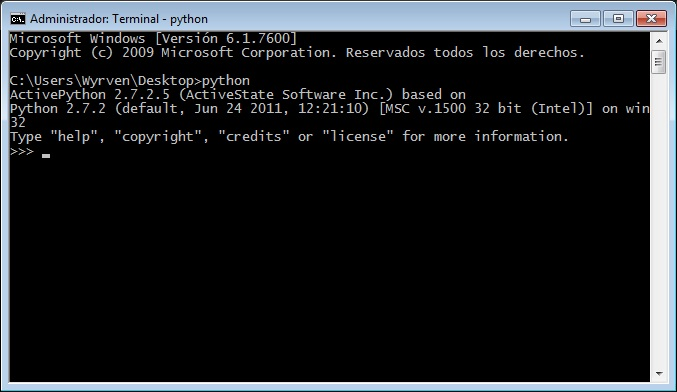
\includegraphics[scale=0.7]{resourse/consola-python.jpg}
    \caption{Ejecutando Python en la Terminal}
    \label{fig:01}
\end{figure}    

En caso contrario deberias revisar que la ruta de Python este dentro de la variable
 PATH del sistema.





\section{Django}

Django es un framework de desarrollo web de código abierto, escrito en Python,
que respeta el paradigma conocido como {\bfseries Model Template View}. Fue desarrollado en
origen para gestionar varias páginas orientadas a noticias de la
{\bfseries World Company de Lawrence, Kansas}, y fue liberada al público bajo una licencia
BSD en julio de 2005; el framework fue nombrado en alusión al guitarrista de
jazz gitano Django Reinhardt \url{http://es.wikipedia.org/wiki/Django_Reinhardt}.

En junio del 2008 fue anunciado que la recién formada Django Software Foundation
se haría cargo de Django en el futuro.

La meta fundamental de Django es facilitar la creación de sitios web complejos.
Django pone énfasis en el re-uso, la conectividad y extensibilidad de
componentes, el desarrollo rápido y el principio No te repitas
(DRY, del inglés Don't Repeat Yourself). Python es usado en todas las partes
del framework, incluso en configuraciones, archivos, y en los modelos de datos.


\subsection{MVC}

Antes de Explicar como funciona Django empezare por una breve explicacion de
el patr\'on (MVC) Modelo Vista Controlador el cual es un patrón de arquitectura de software que
separa los datos y la lógica de negocio de una aplicación de la interfaz de
usuario y el módulo encargado de gestionar los eventos y las comunicaciones.
Para ello MVC propone la construcción de tres componentes distintos que son el
modelo, la vista y el controlador, es decir, por un lado define componentes
para la representación de la información, y por otro lado para la interacción
 del usuario. Este patrón de diseño se basa en las ideas de reutilización de
 código y la separación de conceptos, características que buscan facilitar la
 tarea de desarrollo de aplicaciones y su posterior mantenimiento.

De manera genérica, los componentes de MVC se podrían definir como sigue:

{\bfseries  El Modelo:} Es la representación de la información con la cual el sistema opera,
por lo tanto gestiona todos los accesos a dicha información, tanto consultas
como actualizaciones, implementando también los privilegios de acceso que se
hayan descrito en las especificaciones de la aplicación (lógica de negocio).
Envía a la 'vista' aquella parte de la información que en cada momento se le
solicita para que sea mostrada (típicamente a un usuario). Las peticiones de
acceso o manipulación de información llegan al 'modelo' a través del
'controlador'.

{\bfseries El Controlador: } Responde a eventos (usualmente acciones del
usuario) e invoca peticiones al 'modelo' cuando se hace alguna solicitud sobre
la información (por ejemplo, editar un documento o un registro en una base de
datos). También puede enviar comandos a su 'vista' asociada si se solicita un
cambio en la forma en que se presenta de 'modelo' (por ejemplo, desplazamiento
 o scroll por un documento o por los diferentes registros de una base de datos),
  por tanto se podría decir que el 'controlador' hace de intermediario entre
   la 'vista' y el 'modelo' actuando como Middleware
\footnote{Middleware es el software que proporciona un enlace entre aplicaciones de software
independientes. Middleware a veces se llama a la vía que conecta dos
aplicaciones y pasa los datos entre ellas. Los Middleware permiten que los
datos contenidos en una base de datos puedan ser accedidos a través de otra.
Ahorra el tiempo a los programadores.}.
   
{\bfseries La Vista: } Presenta el 'modelo' (información y lógica de negocio)
 en un formato adecuado para interactuar (usualmente la interfaz de usuario)
 por tanto requiere de dicho 'modelo' la información que debe representar como
 salida.

\begin{figure}[h]
    \centering
    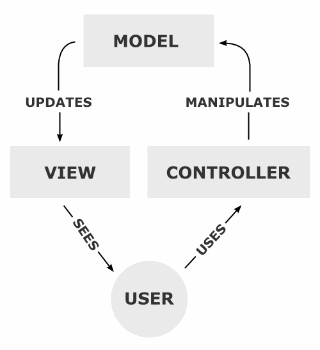
\includegraphics[scale=0.7]{resourse/MVC-Process.png}
    \caption{Diagrama del Patron MVC Modelo Vista Controlador}
    \label{fig:03}
\end{figure}    


\subsection{Django y el MVT}

Si hicieramos una clasificacion de Herramientas de desarrollo web, podriamos
clasificar a Django como parte de la tercera generacion:


\begin{figure}[h]
    \centering
    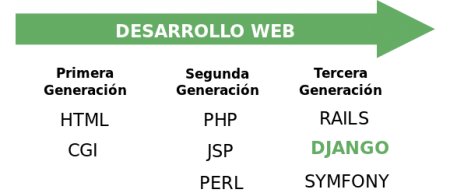
\includegraphics[scale=0.7]{resourse/desarrolloweb.png}
    \caption{Generaciones de Herramientas de Desarrollo Web}
    \label{fig:02}
\end{figure}   

Sin embargo más alla de las clasificaciones que podr\'ian existir, está el
entender como funciona realmente, al entenderlo se puede llegar a dominarlo.

Dijimos que era un framework MTV (una modificación de MVC, nada que ver con
un canal de m\'usica), esto se debe a que los desarrolladores no tuvieron la
 intención de seguir algún patron de desarrollo, sino hacer el framework lo
más funcional posible.

\begin{itemize}
    \item {\bfseries  El Modelo} en Django sigue siendo el modelo
    \item {\bfseries La Vista} en Django se llama Plantilla (Template)
    \item {\bfseries El controlador} en Django se llama Vista
\end{itemize}

Una imagen nos hará entender mejor esta relación:

\begin{figure}[h]
    \centering
    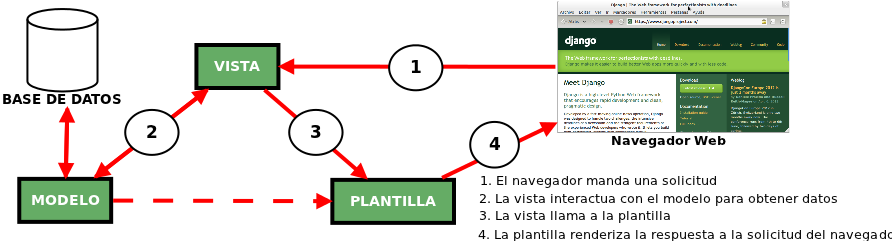
\includegraphics[scale=0.5]{resourse/esquema-mtv.png}
    \caption{El patron Modelo Vista Template de Django}
    \label{fig:04}
\end{figure}   



\subsection{El Modelo}
El modelo define los datos almacenados, se encuentra en forma de clases de
Python, las clases definidas son traducidas por Django y este genera las Tablas
necesarias para el funcionamiento del modelo dentro de la base de datos, cada
tipo de dato que debe ser almacenado se encuentra en una variable 
con ciertos parámetros, posee métodos también. Todo esto permite indicar y
controlar el comportamiento de los datos.\\[0.1cm]

Aqui un extracto del codigo mostrando como se implementa uno de los tantos
modelos con los que trabaja el Sistema\\[0.3cm]


\begin{lstlisting}[style=Python]

class Message(models.Model):
    """
        Clase Para Manejar mensajes entre usuarios
    """
    from_user = models.ForeignKey(User, related_name='from_user')
    to_user = models.ForeignKey(User, related_name='to_user')
    date = models.DateTimeField("Fecha y Hora",auto_now_add=True)
    issue = models.CharField("Asunto",max_length=125, default='')
    content = models.TextField("Cuerpo del Mensaje")
    read = models.BooleanField("Leido",default=False)


    class Meta:
        db_table = "Messages"
        verbose_name = "InboxMessage"
        verbose_name_plural = "InboxMessages"
\end{lstlisting}

\footnote{Como algunos lo notaran la variable from\_user del modelo internamente
es una relacion 1:M dentro de la base de datos.}

\footnote{La Clase interna Meta define atributos expeciales como 'db\_name' que hace
referencia a como se llamara la tabla dentro de la Bases de Datos.}

\vspace{0.1cm}

\subsection{La Vista}
La vista se presenta en forma de funciones en Python, su propósito es
determinar que datos serán visualizados, entre otras cosas más que iremos
viendo conforme avanzamos con el curso. El ORM de Django permite escribir
código Python en lugar de SQL para hacer las consultas que necesita la vista.
La vista también se encarga de tareas conocidas como el envío de correo
electrónico, la autenticación con servicios externos y la validación de
datos a través de formularios. Lo mas importante a entender con respecto a la
 vista es que no tiene nada que ver con el estilo de presentación de los
 datos, sólo se encarga de los datos, la presentación es tarea de la plantilla.\\[0.1cm]


Aqui muestro una vista sencilla que realiza una consulta base de datos que listara todos
los usuarios que sean medicos. \\[0.1cm]

\begin{lstlisting}[style=Python]
def patient_show_medics_list(request):
    """
        Muestra el listado de Medicos
    """
    mi_template = get_template('Patients/GestionTurnos/medics-list.html')
    dict = generate_base_keys(request)

    if is_patient(request.user):
        dict['medics'] = UserInformation.objects.filter( \\
                                    user__groups__name='Medico')
        html_cont = mi_template.render(Context(dict))
        return HttpResponse(html_cont)

    else:
        #si hay un usuario logueado intentanto acceder sera enviado a una
        # pagina de error
        path = request.META['PATH_INFO']
        return HttpResponseRedirect("/restricted-access%s" %path)
\end{lstlisting}

\vspace{0.1cm}

Aunque es un ejemplo sencillo podemos apreciar el potencial de Django, como vemos
no vemos ningun codigo SQL, pues bien dicho codigo SQL se ejecuta internamente
nos aleja del problema de las restriciones de la Base de Datos ya sea que usemos
PosgreSQL (como en este sistema), MySQL, SQLServer o SQLite nosotros
solo escribiremos codigo Python, El framework se encargargara de traducir esa
instrucion al motor de bases de datos correspondiente que estemos usando.\\[0.2cm]

\begin{lstlisting}[style=consola]
dict['medics'] = UserInformation.objects.filter( \\
                            user__groups__name='Medico')
\end{lstlisting}

\vspace{0.1cm}

Traducido a SQL terminariamos con algo tan orrible como esto:\\[0.1cm]

\begin{lstlisting}[style=consola]
SELECT * FROM UserInformation as Info
INNER JOIN User ON Info.username = User.username
INNER JOIN GroupsByUsers ON User.username = GroupsByUsers.username
...
\end{lstlisting}

\vspace{0.1cm}

\subsection{La Plantilla}
La plantilla es básicamente una página HTML con algunas etiquetas extras
propias de Django, en si no solamente crea contenido en HTML (también XML, CSS,
Javascript, CSV, etc).\\[0.1cm]

La plantilla recibe los datos de la vista y luego los organiza para la
presentación al navegador web. Las etiquetas que Django usa para las plantillas
permiten que sea flexible para los
diseñadores del frontend, pueden Extenderse a partir de otras plantillas incluso
tiene estructuras de datos como if, por por si es necesaria una presentación
lógica de los datos, estas estructuras
son límitadas para evitar un desorden poniendo cualquier tipo de código Python.\\[0.1cm]

Esto permite que la lógica del sistema siga permaneciendo en la vista. Aqui la
vista para Iniciar Session:\\[0.1cm]

\begin{lstlisting}[style=HTML]



<link type="text/css" rel="stylesheet" media="all"
    href="/media/css/fancy-forms.css" />
<link type="text/css" rel="stylesheet" media="all"
    href="/media/css/gradient-buttons.css" />
<link type="text/css" rel="stylesheet" media="all"
    href="/media/css/messages.css" />




<br /><br /><br />
        
            <div class="fancy-form-white" style="width: 350px;
                margin: 0 auto;">
                <h3 class="title">Inciar Session</h3><br />
                <form action="." method="POST">
                <table style="margin: 0 auto; width: 330px;" >
                <tr>
                    <td><label for="username">Usuario:</label></td>
                    <td><input type="text" name="username" value=""
                    tabindex="1" id="username"></td>
                    <td rowspan="2">
                    <input type="submit" value="Login" tabindex="3"
                    class="grad-button-blue" style="height: 50px;">
                    </td>
                </tr>
                <tr>
                    <td><label for="password">Contrase\~na:</label></td>
                    <td><input type="password" name="password" value=""
                     tabindex="2" id="password"></td>
                </tr>
                </table>
                </form>
                <br />
            </div>

            
                    <br />
                    <br />
                <div class="alert">Alerta: Error Usuario y/o Contrase\~na
                Incorrectos</div>
            

        
            <div class="alert">Alerta: Usted ya ha iniciado session con el
            usuario <strong>{{ username }}</strong></div>
            <br />
            <a href="/logout">Cerrar Session</a>
        

\end{lstlisting}

\vspace{0.1cm}

\subsection{La Configuracion de Rutas}

Django posee un mapeo de URLs que permite controlar el despliegue de las vistas,
esta configuración es conocida como URLConf. El trabajo del URLConf es leer
la URL que el usuario solicitó, encontrar la vista apropiada para la solicitud
y pasar cualquier variable que la vista necesite para completar su trabajo. El
URLConf esta construido con expresiones regulares en Python y sigue la filosofia
de Python: Explicito es mejor que implícito. Este URLConf permite que las rutas
que maneje Django seán agradables y entendibles para el usuario.\\[0.1cm]

Fragmento del archivo urls.py del Proyecto\\[0.1cm]

\begin{lstlisting}[style=HTML]
    (r'^$', base_views.index),
    (r'^index/$', base_views.index),
    (r'^login/$', base_views.login),
    (r'^logout/$', base_views.logout),
    (r'^change-password/$', base_views.change_password),
    (r'^restricted-access/$', base_views.restricted_access),
    (r'^restricted-access/(.+)/$', base_views.restricted_access),
\end{lstlisting}

\vspace{0.1cm}


\subsection{Instalar Django}

Puedes bajarte Django desde el siguiente enlace \url{https://www.djangoproject.com/download/1.3.7/tarball/}
\footnote {la version 1.3.7 no es la ultima version disponible a la hora de crear
este informe estaba por la 1.6.2 ya que Django se actualiza constantemente.}
te descargara un paquete llamado Django-1.3.7.tar.gz lo descomprimes en
algun directorio luego abres la Terminal y te posicionas sobre el directorio
donde descomprimiste y ejecutas:

\begin{lstlisting}[style=consola]
    $ python setup.py install 
\end{lstlisting}
\vspace{0.1cm}

Sino mediante el instalador de Paquetes de Python de manera mas automatica escribes
en la terminal

\begin{lstlisting}[style=consola]
     pip install django==1.3.7
\end{lstlisting}
\vspace{0.1cm}

Con esto ya tendremos instalado Django.

\section{Instalando el Resto de Las Dependencias}

Ademas de Django en el Proyecto se utilizaron otras Librerias de Python las cuales
algunas vienen instaladas y Otras Requieren ser instaladas de manera similar
a como instalamos Django.

\subsection{psycopg2}

psycopg2 es un adaptador de base de datos PostgreSQL para el lenguaje de
programación Python. psycopg2 fue escrito con el objetivo de ser muy pequeño
y rápido y estable. 

psycopg2 es diferente del otro adaptador de base de datos, ya que fue diseñado
para aplicaciones en gran medida de subprocesos múltiples que crean y destruyen
un montón de cursores y hacen que un número notable de inserciones o
actualizaciones concurrentes. psycopg2 también proporcionan operaciones
asincrónicas completos y apoyo a las bibliotecas de co-rutinas. 

Para instalar descargue el precompilado desde \url{http://www.stickpeople.com/projects/python/win-psycopg/}
Ejecutelo con permisos de administrador, nos pedira que selecionemos la version
de python con que se instalar.

\subsection{ReportLab}

ReportLab es la ultra-robusto motor de código abierto a prueba de tiempo para
la creación de documentos PDF y gráficos vectoriales personalizado. Escrito en
Python, ReportLab es rápido, flexible y una plataforma cruzada.
 
Proporciona un completo conjunto de herramientas de programación para la
creación de documentos y gráficos complejos. Ofrecemos una serie de componentes
 de forma gratuita y de código abierto, además de un paquete comercial con
características adicionales.

Para Instalar descargue el instalado desde \url{http://www.reportlab.com/software/installation/}
y proceda de manera similar a como hizo con la instalacion de psycopg2.


\subsection{easy\_thumbnails}


\subsection{django\_extensions}


\subsection{django\_cron}

Django-cron permite ejecutar código de Django de manera recurrente para el
seguimiento y ejecución de las tareas. En este caso no es Necesario Instalar
Nada, viene junto con el Codigo Fuente del Proyecto. Igualmente si tiene curiosidad
puede visitar la pagina del proyecto \url{https://github.com/Tivix/django-cron}





\section{mod\_wsgi}

mod\_wsgi es un módulo de Apache que provee una interfaz WSGI para correr
 Web en Python sobre Apache. Y esto, es todo lo que necesitas para que tus
 archivos *.py se ejecuten por medio de un navegador Web.

\subsection{WSGI}

WSGI es el acronomico de Web Server Gateway Interface que es una especificacion
para una simple y universal interfaz entre una aplicacion web (en nuestro caso
una aplicacion escrita en Django) y un servidor Web para el lenguaje de programacion
Python. Es un estandar de Python el cual se describe con detalle en la PEP 333
\footnote{\url{http://www.python.org/dev/peps/pep-0333/}}


\subsection{Descargar e Instalacion}

 Asumiendo que ya  tienes instalado Python y Apache, solo debes descargar el paquete
 libapache2-mod-wsgi ,la ultima version de mod\_wsgi se puede descargar desde su
 pagina oficial \url{https://code.google.com/p/modwsgi/} descargaran un archivo
 similar a "mod\_wsgi-win32-ap22py27-3.3.so" la version que descarguen de mod\_wsgi
 depende como se ve, de la plataforma asi como de la version de python que
 correrar en el servidor. luego por cuestiones de practicidad renombraremos
 el archivo de la siguiente manera:

\begin{lstlisting}[style=consola]
    mod_wsgi-win32-ap22py27-3.3.so -> mod_wsgi.so
\end{lstlisting}
\vspace{0.1cm}

Realizado dicho cambio copiamos el modulo dentro de la siguiente carpeta:
APACHE\_FOLDER \textbackslash modules \textbackslash APACHE\_FOLDER vendria a
ser el directorio donde tenemos la instalacion de WAMP en mi caso es:
C:\textbackslash Apache.

\subsection{Cargando el Modulo en Apache}

Una vez que el módulo de Apache ha sido instalado en el directorio de módulos
de su instalación de Apache, todavía es necesario configurar Apache para cargar
el módulo en realidad.

Abrimos el archivo "httpd.conf" y agregamos la siguiente linea en el mismo
punto donde se cargan el resto de los modulos. \footnote {El archivo httpd.conf
esta en la siguiente ruta en el caso de mi instalacion:
C:\textbackslash Apache \textbackslash conf \textbackslash httpd.conf}

\begin{lstlisting}[style=consola]
    LoadModule wsgi_module modules/mod_wsgi.so
\end{lstlisting}
\vspace{0.1cm}

Con todo esto echo solo tenemos que reiniciar el servidor Apache, en nuestro
 caso clic en el icono en la barra de notificaciones luego las opciones
 Apache->Service->Reiniciar Servicio. 

\subsection{Configuracion del Proyecto}

Bueno Ahora solo tenemos que crear un alias en Apache \footnote{Para mayor
informacion de como crear alias en Apache consulte
\url{http://httpd.apache.org/docs/2.2/urlmapping.html}} para nuestra carpeta
donde colocaremos en mi caso la carpeta destino sera:

\begin{lstlisting}[style=consola]
	C:\Servidor\SGCM
\end{lstlisting}
\vspace{0.1cm}

SGCM es la carpeta contenedora del proyecto, y el alias que usaremos sera:

\begin{lstlisting}[style=consola]
	/sgcm/ 
\end{lstlisting}
\vspace{0.1cm}

tendremos que agregar las siguientes lineas al final del archivo
httpd.conf de apache.

\begin{lstlisting}[style=HTML]
Alias /sgcm/ "C:/Servidor/SGCM/" 
WSGIScriptAlias /sgcm "C:/Servidor/SGCM/handle.wsgi" 

<Directory "C:/Servidor/SGCM">
    Options Indexes FollowSymLinks MultiViews
    AllowOverride all
    Order allow,deny
    Allow from all
</Directory>
\end{lstlisting}
\vspace{0.1cm}



Hay un número de maneras en que una aplicación WSGI organizada por mod\_wsgi
\footnote{Puede consultar \url{https://code.google.com/p/modwsgi/wiki/QuickInstallationGuide}
si desea explorar otras opciones de configuracion.}
puede montarse contra una URL específica. Estos métodos son similares a cómo se
podría configurar las aplicaciones CGI tradicionales.

El principal enfoque implica declarar explícitamente en el archivo de
configuración principal de Apache el punto de montaje URL y una referencia al
archivo de comandos de aplicaciones WSGI. En este caso, el mapeo se fija,
con cambios sólo ser capaz de ser hecho mediante la modificación de la
configuración principal de Apache y reiniciar Apache.

Al utilizar mod\_cgi para alojar aplicaciones CGI, esto se haría mediante la
directiva ScriptAlias. Para mod\_wsgi, la directiva en su lugar se
llama WSGIScriptAlias.

\begin{lstlisting}[style=consola]
WSGIScriptAlias /wsgi "C:/Servidor/SGCM/handle.wsgi" 
\end{lstlisting}
\vspace{0.1cm}

Esta directiva s\'olo puede aparecer en los principales archivos de configuración
de Apache. La directiva se puede utilizar en el ámbito del servidor, pero
normalmente se coloca en el contenedor VirtualHost para un sitio en particular.
No se puede utilizar en cualquiera de las directivas de contenedores ubicación,
directorios o archivos, ni puede ser utilizada dentro de un archivo ''.httaccess''.

El primer argumento de la directiva WSGIScriptAlias debe ser el punto de montaje
URL para la aplicación WSGI. En este caso, la URL no debe contener una barra
diagonal. La única excepción a esto es si la aplicación WSGI es para ser
montado en la raíz del servidor web, en cuyo caso / sería utilizado.

El segundo argumento de la directiva WSGIScriptAlias debe ser una ruta absoluta
para el archivo de comandos de aplicaciones WSGI. Es en este archivo que la
muestra de código de la aplicación WSGI debe colocarse.

Tenga en cuenta que una ruta absoluta debe ser utilizado para el archivo de
comandos de aplicaciones WSGI suministrado como segundo argumento. No es posible
especificar una aplicación por sí sola Python nombre de módulo. Una ruta de
acceso completa se utiliza para una serie de razones, la principal de las
cuales por lo que todos los controles de acceso de Apache todavía pueden aplicarse
para indicar que en realidad puede acceder a la aplicación WSGI.

Porque se aplicarán los controles de acceso de Apache, si la aplicación WSGI se
 encuentra fuera de los directorios que ya están configurados para ser accesible a
  Apache, habrá que decirle a Apache que los archivos dentro de ese directorio se
  pueden utilizar. Para ello se debe utilizar la directiva Directory.

Hasta aqui tenemos mod\_wsgi y nuestro directorio listo, ahora probaremos que
todo va bien para ello dentro del directorio crearemos un archivo llamado
"handle.wsgi" que tendra el siguiente contenido:

\begin{lstlisting}[style=Python]
# -*- coding: utf-8 -*-

import os, sys
import django.core.handlers.wsgi

sys.path.append('C:/Servidor/SGCM')
sys.path.append('C:/Servidor')

os.environ['DJANGO_SETTINGS_MODULE'] = 'settings'

application = django.core.handlers.wsgi.WSGIHandler()

\end{lstlisting}
\vspace{0.1cm}


Con esto nuestro servidor de aplicacion ya deberia funcionar aunque como veran
no se cargan los archivos estaticos como imagenes y hojas de estilo por lo
que necesitamos agregarlo.

%%%




\part*{\addcontentsline{toc}{part}{Apéndices}Apéndices}

% Adjustments headers
\fancyhead[RO]{\leftmark}
\fancyhead[EL]{\emph{Apéndice \thechapter}}

%%%%%%%%%%%%%
\appendix
%%%%%%%%%%%%%%
%\ include{software}
%\ include{publicaciones}


%%%%%%%%%%%%%
\backmatter
%%%%%%%%%%%%%
% Adjustments headers
\fancyhead[RO]{\leftmark}
\fancyhead[EL]{}
\addcontentsline{toc}{chapter}{Bibliografía}
\bibliographystyle{unsrt}
%\bibliography{lmm,gengisNOlmm}
%\printindex
\end{document}

%%% Local Variables: 
%%% mode: latex
%%% TeX-master: "tesis"
%%% End: 
